%-------------------------------------------------------------------------------
%
%     CHARGEMENT DES EXTENSIONS
%
%-------------------------------------------------------------------------------

\documentclass[11pt,fleqn]{report}
\usepackage{GarmirKhatch}
\usepackage{MjMcd}

\definecolor{colone}{RGB}{209,220,204}
\definecolor{coltwo}{RGB}{204,222,210}
\definecolor{colthree}{RGB}{207,233,232}
\definecolor{colfour}{RGB}{248,243,214}
\definecolor{colfive}{RGB}{245,238,197}
\definecolor{colsix}{RGB}{243,235,179}
\definecolor{colseven}{RGB}{241,231,163}


%-------------------------------------------------------------------------------
%     Informations spécifiques au document
%-------------------------------------------------------------------------------

\ZTitle{Système de gestion des transports}
\ZSubject{Procédure de génération de tables SQL avec JMerise}
\ZVersion{1.0}
\ZDate{\today}


%-------------------------------------------------------------------------------
%     Contenu
%-------------------------------------------------------------------------------

\begin{document}

\ZMakeCover

\ZMakeInformations{
	% Historique des modifications
	% Version & Date & Auteur(s) & Modification(s)
	1.0 & 2014-03-06 & \Gairoard & Rédaction \\
}{
	% Historique des approbations
	% Version & Date & Approbateur(s)
	1.0 & - & - \\
}{
	% Historique des validations
	% Version & Date & Responsable(s)
	1.0 & - & - \\
}

\ZMakeTableOfContents

\section{Présentation}
JMerise est un logiciel dédié à la modélisation des modèles conceptuels de donnée pour Merise. Il permet en autre, les relations réflexives, la généralisation et la spécialisation des entités. Il génère le MLD et le script MySQL associé.

\section{Procédure d'installation}
Pour installer et utiliser JMerise, dezipper simplement le fichier "\textbf{JMerise.zip}" et exécuter le jar nommé "\textit{JMerise.jar}". 

\section{Procédure de génération de génération de tables SQL}
Une fois la MCD réalisée, JMerise propose une méthode de vérification qui permet de s'assurer que le modèle que l'utilisateur vient de créer est correct. Pour cela, il suffit de cliquer sur le bouton 
\includegraphics[scale=0.35]{checkMCD}.\\
L'outil peut aussi générer la MPD associée ainsi que le code MySQL permettant la création des tables en cliquant sur le bouton 
\includegraphics[scale=0.35]{convertMCD}.

\begin{figure}
\begin{center}
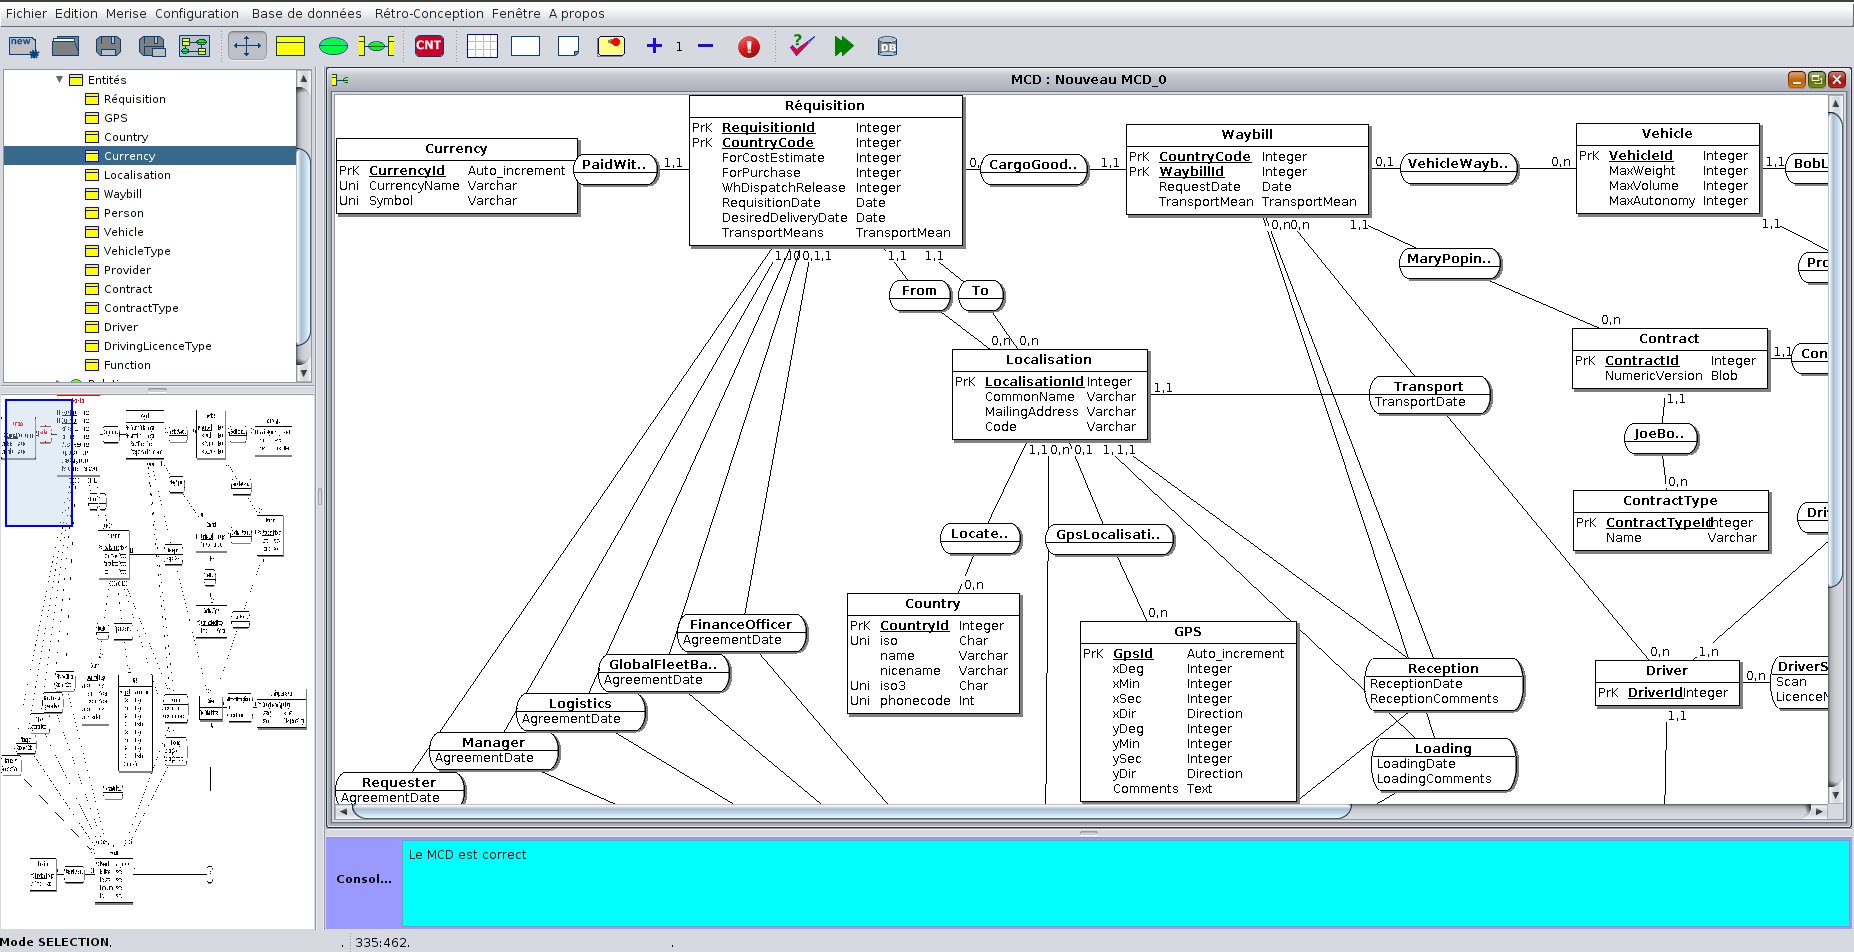
\includegraphics[scale=0.25]{jmerise}
\end{center}
\caption{Exemple de MCD avec JMerise}
\end{figure}

% TODO : À terminer


% Affichage de la liste des figures
\newpage
\listoffigures

% Affichage de la liste des tableaux
%\newpage
%\listoftables

\end{document}
